%%% template.tex
%%%
%%% This LaTeX source document can be used as the basis for your technical
%%% paper or abstract. Intentionally stripped of annotation, the parameters
%%% and commands should be adjusted for your particular paper - title, 
%%% author, article DOI, etc.
%%% The accompanying ``template.annotated.tex'' provides copious annotation
%%% for the commands and parameters found in the source document. (The code
%%% is identical in ``template.tex'' and ``template.annotated.tex.'')

\documentclass[conference, 12pt]{acmsiggraph}

\title{Reconstructing scenes from photos using Global SfM}

\author{Bryce Evans \and Rafael Farias Marinheiro}
% \contactemail{}
\affiliation{Cornell University\thanks{\{bae43, rf356\}@cornell.edu}}
\pdfauthor{Rafael F. Marinheiro}

\keywords{crowd simulation, user interaction, real-time rendering}

\usepackage{amsmath}


\begin{document}

%% \teaser{
%%   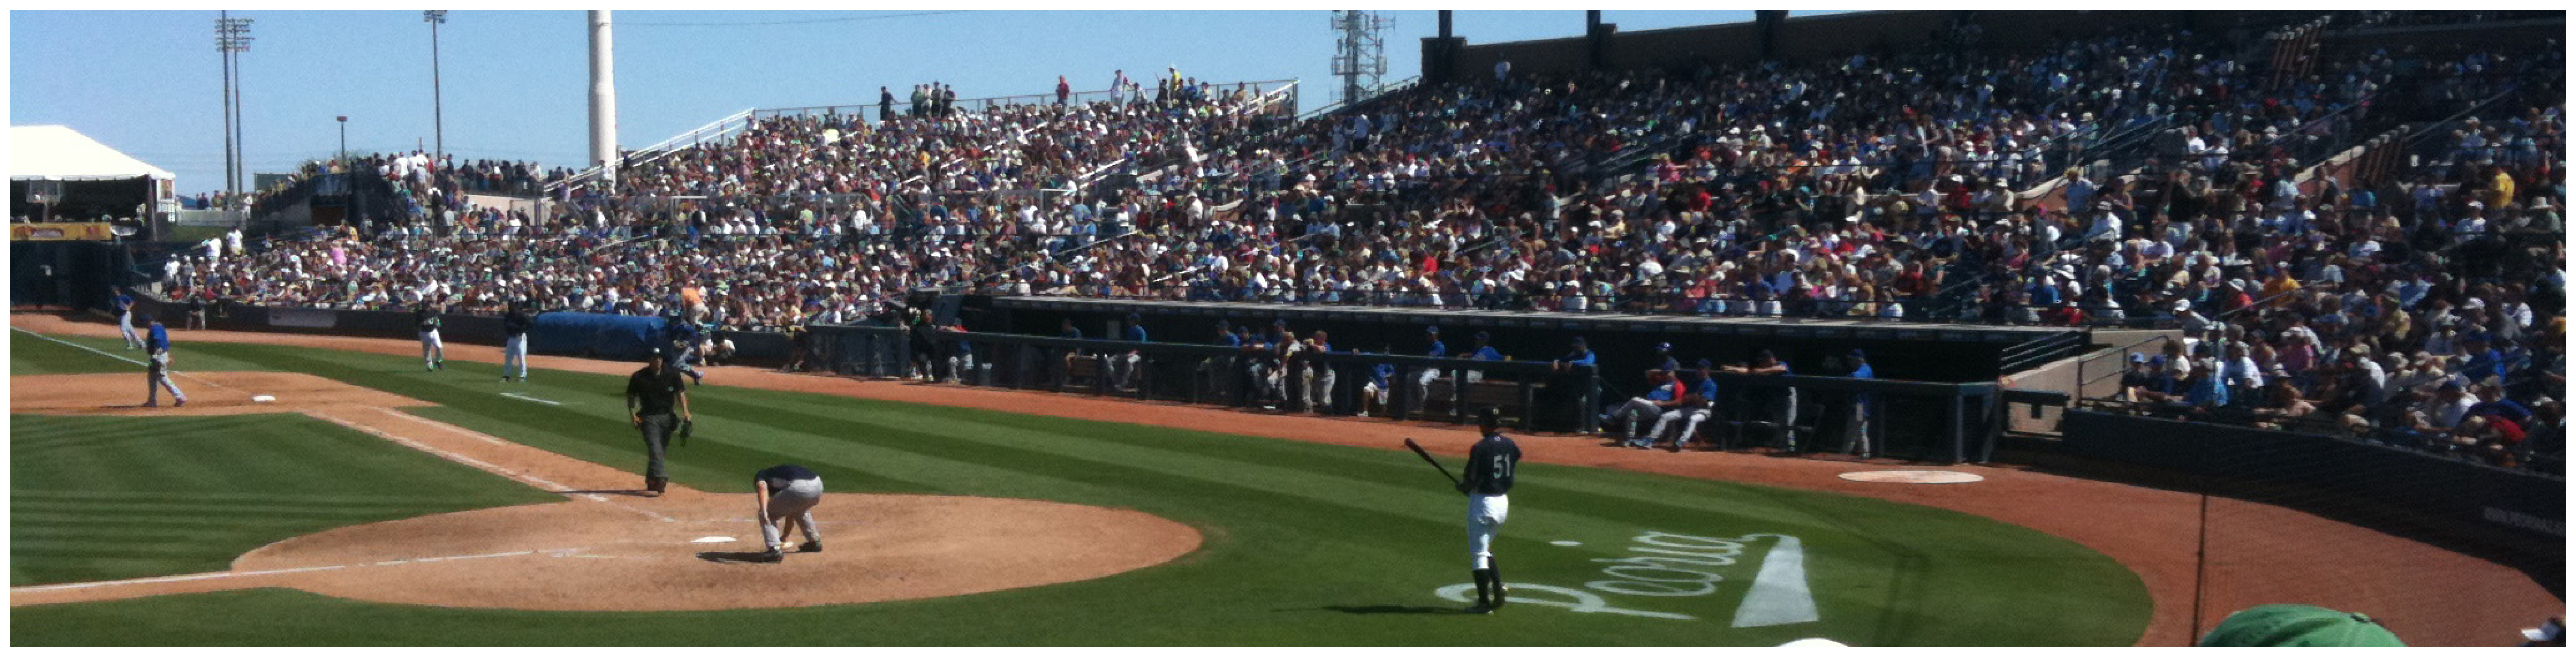
\includegraphics[height=1.5in]{images/sampleteaser}
%%   \caption{Spring Training 2009, Peoria, AZ.}
%% }

\maketitle

% \begin{abstract}

% We intend to create a interactive Crowd Simulation application using the approach described in \cite{kim2012interactive}. The user will be able to interact with the application with a commodity depth sensor \cite{Zhang:2012:MKS:2225053.2225203}, modifying the environment in real time.

% \end{abstract}

% \begin{figure}[Ht!]
%   \centering
%     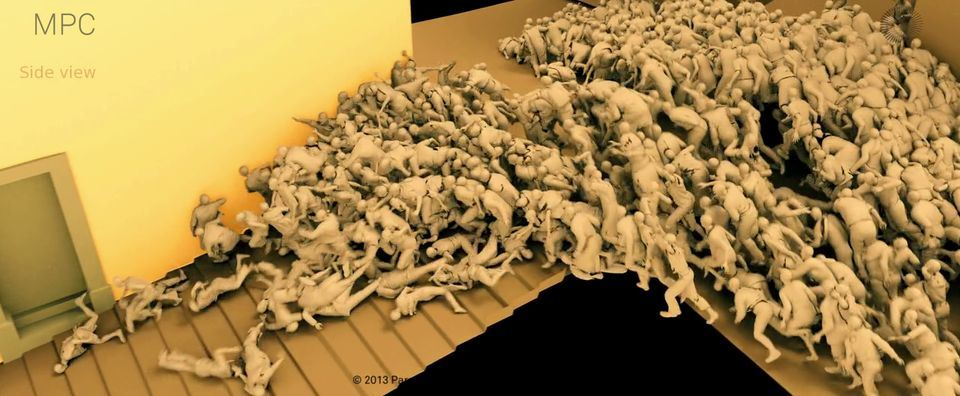
\includegraphics[width=0.5\textwidth]{images/mpc3.jpg}
%     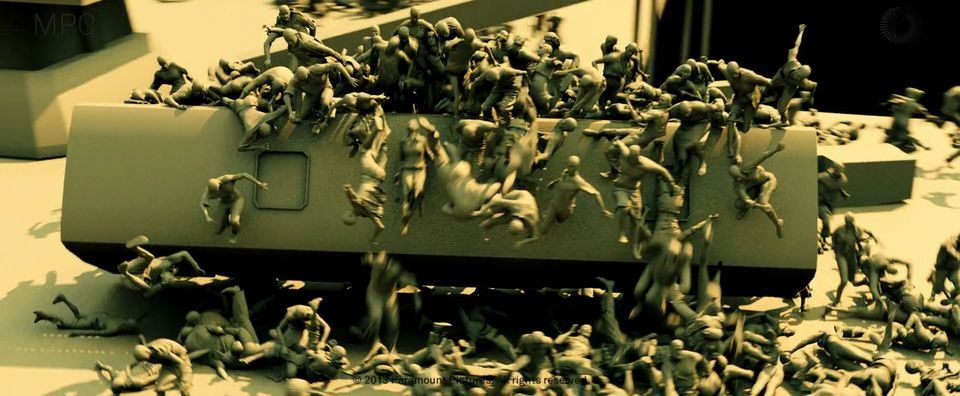
\includegraphics[width=0.5\textwidth]{images/mpc2.jpg}
% 	\caption{World War Z (2013). Zombie agents were computationally simulated.}
% 	\label{fig:wwz}
% \end{figure}

% %% Use this only if you're preparing a technical paper to be published in the 
% %% ACM 'Transactions on Graphics' journal.

% \begin{CRcatlist}
% 	\CRcat{I.2.11}{Artificial Intelligence}{Distributed Artificial Intelligence}{Multiagent systems};
% 	\CRcat{I.3.7}{Computer Graphics}{Three-Dimensional Graphics and Realism}{Animation};
% 	\CRcat{I.6.8}{Simulation and Modeling}{Types of Simulation}{Animation}
% \end{CRcatlist}

% %%% The ``\keywordlist'' prints out the user-defined keywords.

% \keywordlist

% \TOGlinkslist

% %% Required for all content. 

% \copyrightspace

\section{Problem}

Large image sets are around us everyday but give little understanding into the scenes they are of. Making use of data to create 3D geometry could give strong representations of buildings for navigating cities or reconstructing objects to save modeling time. Applications such as Google Maps make use of these large image sets to reconstruct landscapes, but making a system more robust for disorganized sets and generalized to generating a 3D mesh for any geometry would have greater application.

In this project, we pretend to implement parts of a Structure From Motion Pipeline. We will assume that cameras correspondences are given as an input and then we will try to reconstruct the image from that. More specifically, we are trying to solve the problem described as follows: Consider a connected graph $G = (V,E)$. Associated with each edge $e = (i, j)$, there is a relative rotation $R_{ij} \in SO(3)$ and relative translation $T_{ij} \in R^3$. We want to assign to each vertex of the graph a global rotation and translation $R_i, T_i$ such that we minimize:

\begin{eqnarray}
	\sum_{(i,j) \in E} d_1(R_{j}R_{i}^{-1}, R_{ij}) \\
	\sum_{(i,j) \in E} d_2(T_{j}-T_{i}, T_{ij})
\end{eqnarray}

Where $d_1$ and $d_2$ are metrics of $SO(3)$ and $R^3$ respectively. There are two different types of approaches to solve such a problem: The first type of approach, called Iterative SfM, tries to solve this problem for a subset of the graph and then it iteratively adds new cameras. The second type of approach, called the Global SfM, tries to solve for all the nodes at once. Since the rotation problem and the translation problem are independent, one can use different techniques to solve each one.

\section{Goals}

We will implement the technique described by \cite{rotation}. We intend to test it using the datasets published by \cite{rotation} and \cite{translation}. If we have extra time, we might try to build our own dataset.

\section{Schedule}

\subsection{Plan C}

\begin{itemize}
	\item {Week of October 27th}: Read and fully understand \cite{rotation}
	\item {Week of November 3rd}: Implementation
	\item {Week of November 10th}: Implementation
	\item {Week of November 17th}: Testing and Debugging
	\item {Week of November 24th}: Testing and Debugging
	\item {Week of December 1st}: Evaluation
	\item {Week of December 8th}: Evaluation
\end{itemize}


\bibliographystyle{acmsiggraph}
\bibliography{proposal}

\end{document}
